\documentclass[aspectratio=169, 12pt]{beamer}

% ── Theme ─────────────────────────────────────────────────────────────────────
\usetheme{Madrid}
\usecolortheme{seahorse}
\setbeamertemplate{navigation symbols}{}
\setbeamertemplate{footline}[frame number]

% ── Packages ──────────────────────────────────────────────────────────────────
\usepackage{amsmath, amssymb}
\usepackage{graphicx}
\usepackage{booktabs}
\usepackage{xcolor}
\usepackage{tikz}
\usepackage{listings}

\graphicspath{{../../plots/}}   % pull figures from ../plots/

% ── Custom colors (match Python palette) ──────────────────────────────────────
\definecolor{trivial}{HTML}{d62728}
\definecolor{critical}{HTML}{2ca02c}
\definecolor{topological}{HTML}{1f77b4}
\definecolor{edgemode}{HTML}{e377c2}
\definecolor{codebg}{HTML}{f5f5f5}
\definecolor{codekw}{HTML}{0000cd}
\definecolor{codecomment}{HTML}{228b22}
\definecolor{codestring}{HTML}{8b0000}

% ── Code listing style ────────────────────────────────────────────────────────
\lstset{
  language=Python,
  basicstyle=\ttfamily\footnotesize,
  keywordstyle=\color{codekw}\bfseries,
  commentstyle=\color{codecomment}\itshape,
  stringstyle=\color{codestring},
  backgroundcolor=\color{codebg},
  frame=single,
  framerule=0.4pt,
  rulecolor=\color{gray},
  showstringspaces=false,
  breaklines=true,
  tabsize=4,
}

% ── Macros ────────────────────────────────────────────────────────────────────
\newcommand{\cdag}{c^{\dagger}}
\newcommand{\gA}{\gamma_{A,j}}
\newcommand{\gB}{\gamma_{B,j}}
\newcommand{\winding}{\nu}

% ── Title ─────────────────────────────────────────────────────────────────────
\title[Kitaev Chain — Block 2]{Majorana Modes in the Machine}
\subtitle{Block 2: Finite-Size Physics \& Edge Modes}
\author{Dobromir Stoev\\ Edgar Harutyunyan\\ Guilherme Schewtschik\\ Jaskaran Singh\\ Zhengyi Liu\\ Zhenming Shi}
\institute{Advanced Seminar — AI-Augmented Theoretical Physics}
\date{\today}

% ══════════════════════════════════════════════════════════════════════════════
\begin{document}

\begin{frame}
  \titlepage
\end{frame}

% ── Outline ───────────────────────────────────────────────────────────────────
\begin{frame}{Outline}
  \tableofcontents
\end{frame}

% ── Numerical algorithm ───────────────────────────────────────────────────────
\section{Numerical Method}

\begin{frame}[fragile]{Step 1: Building the BdG matrix}
  The real-space BdG Hamiltonian is a $(2L \times 2L)$ block matrix:
  \[
    M = \begin{pmatrix} h & d \\ -d & -h \end{pmatrix}, \quad
    h_{ij} = -\mu\,\delta_{ij} - t(\delta_{i,j+1}+\delta_{i+1,j}), \quad
    d_{ij} = \Delta(\delta_{i,j+1} - \delta_{i+1,j})
  \]

  \begin{lstlisting}
def build_hamiltonian(self):
    h = np.zeros((L, L))
    np.fill_diagonal(h, -mu)          # onsite: chemical potential
    for j in range(L - 1):
        h[j, j+1] = h[j+1, j] = -t   # hopping

    d = np.zeros((L, L))
    for j in range(L - 1):
        d[j, j+1] =  delta            # pairing (antisymmetric)
        d[j+1, j] = -delta

    return np.block([[h, d], [-d, -h]])
  \end{lstlisting}
\end{frame}

\begin{frame}[fragile]{Step 2: Diagonalization \& extracting the spectrum}
  \begin{lstlisting}
def positive_spectrum(self):
    evals = np.linalg.eigvalsh(self.build_hamiltonian())
    return np.sort(np.abs(evals))[:self.L]
  \end{lstlisting}

  \medskip
  \begin{block}{Why \texttt{np.abs} instead of filtering \texttt{evals >= 0}?}
    Particle-hole symmetry guarantees eigenvalues in $\pm E$ pairs.
    Near-zero Majorana modes can round to tiny \emph{negative} values at
    double precision — a sign filter silently drops them, causing spurious
    spikes in the finite-size spectrum at large $L$.
    Taking $|E|$ and keeping the $L$ smallest values is exact.
  \end{block}

  \medskip
  \begin{lstlisting}
# Majorana splitting scan over chain lengths:
E0_arr = np.array([
    np.sort(np.abs(KitaevChain(L=l, ...).spectrum()))[0]
    for l in L_arr
])
  \end{lstlisting}
\end{frame}

% ── Finite-size & edge modes ──────────────────────────────────────────────────
\section{Finite-Size Results}

\begin{frame}{Finite-size spectrum (OBC): edge modes appear}
  \begin{columns}[T]
    \begin{column}{0.65\textwidth}
  \begin{center}
    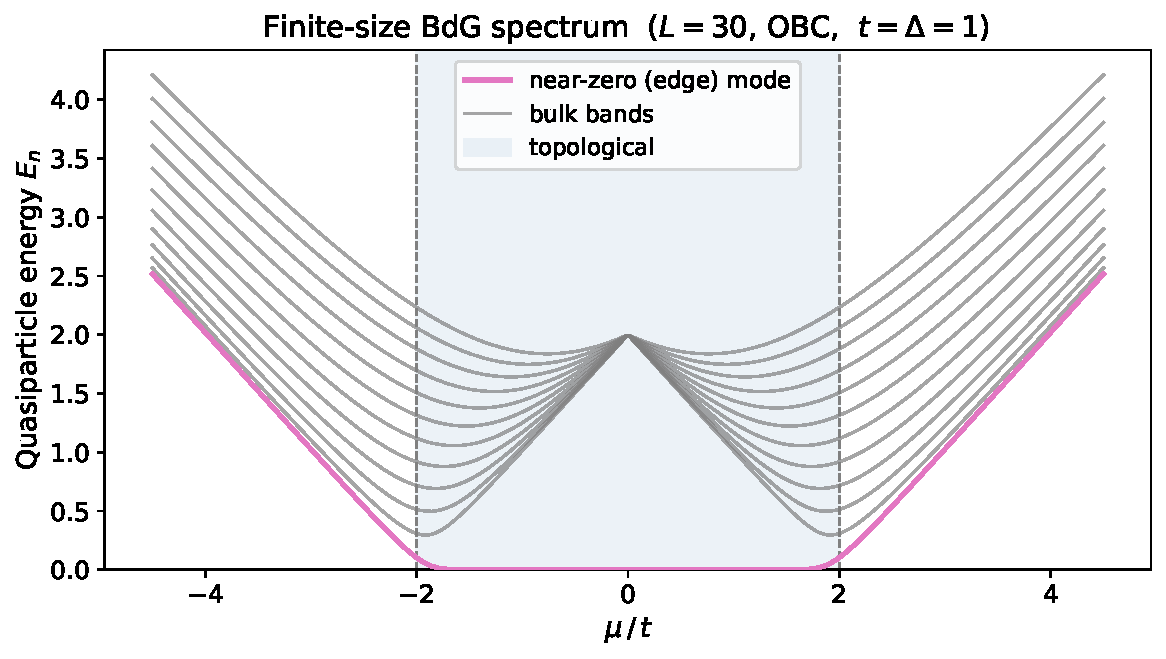
\includegraphics[width=0.9\linewidth]{block1_04_finite_size_spectrum.pdf}
  \end{center}
    \end{column}
    \begin{column}{0.3\textwidth}
    \begin{itemize}  
	 \item {\color{edgemode}Pink} curve: near-zero mode pinned inside the gap across the entire topological phase $|\mu| < 2t$.
     \item  Gray curves: bulk quasiparticle bands — gapped in both phases, closing only at $\mu = \pm 2t$.
    \end{itemize}
	\end{column}
  \end{columns}
\end{frame}

\begin{frame}{Real-space BdG snapshot}
  \begin{center}
    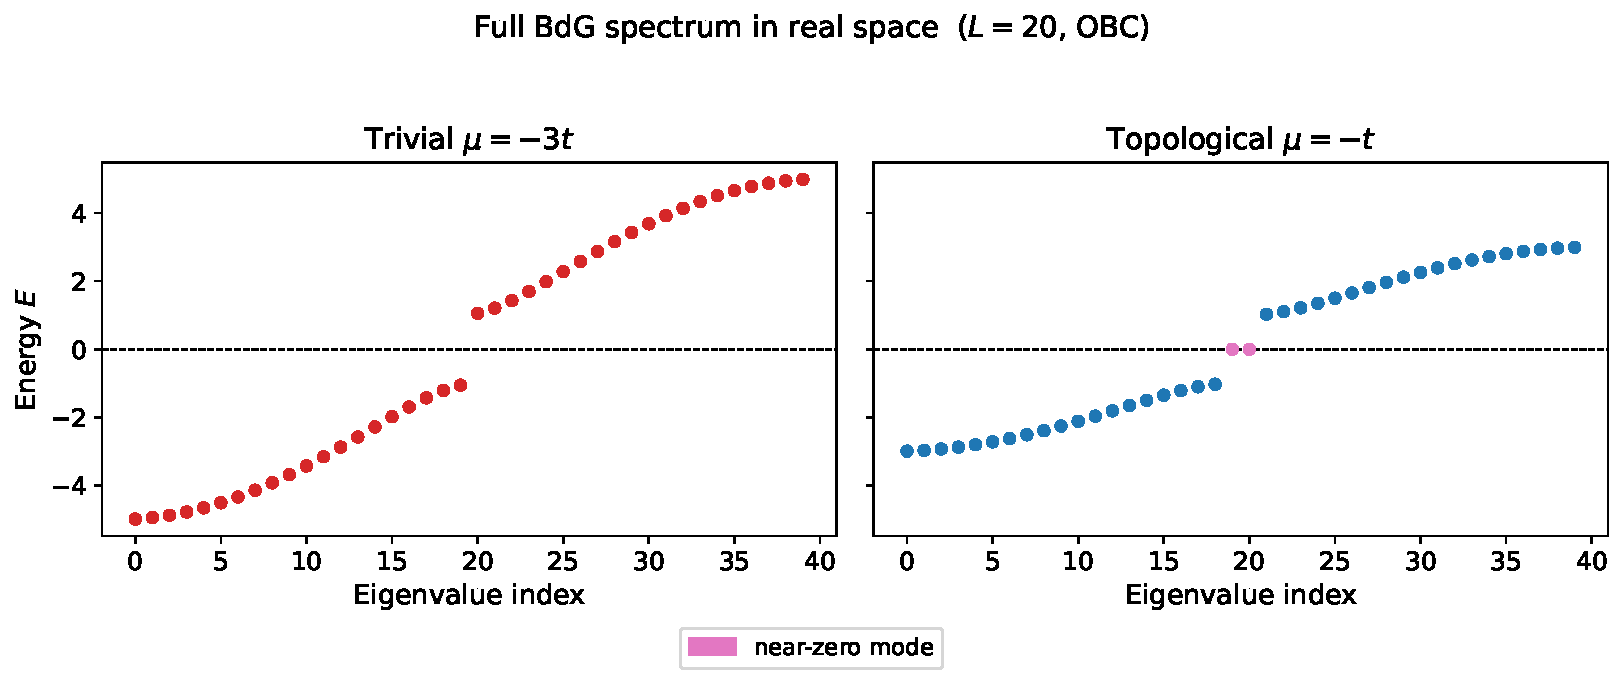
\includegraphics[width=0.82\linewidth]{block1_05_realspace_snapshot.pdf}
  \end{center}
  \textbf{Left} (trivial, $\mu=-3t$): all eigenvalues uniformly gapped — no special states.\\
  \textbf{Right} (topological, $\mu=-t$): two eigenvalues pinned at $E\approx 0$ — the Majorana pair localized at opposite ends of the chain.
\end{frame}

% ── Edge mode localization ────────────────────────────────────────────────────
\section{Edge Mode Localization}

\begin{frame}{Exponential localization of the edge mode}
  At the symmetric point $t = \Delta$, the zero-mode wavefunction has an exact analytical form.
  Substituting the Ansatz $\psi_j \sim \lambda^j$ into the bulk BdG equations gives:
  \[
    \lambda = \frac{\mu}{2t}, \qquad |\lambda| < 1 \text{ (topological phase)}
  \]

  \begin{columns}[T]
    \begin{column}{0.55\textwidth}
      The left edge mode decays as:
      \[
        \psi_j^L \propto \left(\frac{\mu}{2t}\right)^{j-1}
        = e^{-(j-1)/\xi}
      \]
      with coherence length
      \[
        \xi = \frac{1}{\ln(2t/|\mu|)}
      \]
    \end{column}
    \begin{column}{0.42\textwidth}
      \begin{block}{Key points}
        \begin{itemize}
          \item Pure exponential at $t=\Delta$ (no oscillations)
          \item $\xi \to \infty$ as $|\mu| \to 2t$ (phase boundary)
          \item $\xi \to 0$ as $|\mu| \to 0$ (sweet spot)
        \end{itemize}
      \end{block}
    \end{column}
  \end{columns}
\end{frame}

% ── Majorana splitting ────────────────────────────────────────────────────────
\section{Majorana Hybridization Splitting}

\begin{frame}{Derivation: finite-size splitting $E_0(L)$}
  In a \textbf{finite} chain, the left and right edge modes overlap, lifting the degeneracy.
  First-order perturbation theory gives:
  \[
    \delta E = \frac{|\langle \psi^L | H | \psi^R \rangle|}{\|\psi^L\|\,\|\psi^R\|}
  \]

  The overlap is dominated by the mid-chain region:
  \[
    \langle \psi^L | \psi^R \rangle \sim \sum_{j=1}^{L} \lambda^{j-1} \cdot \lambda^{L-j}
    = L\,\lambda^{L-1}
  \]

  Absorbing normalisation and subleading factors into a prefactor fixed by the exact sweet-spot calculation:
  \[
    \boxed{E_0(L) \approx 2t\left(\frac{|\mu|}{2t}\right)^L}
  \]
\end{frame}

\begin{frame}{Majorana hybridization splitting vs system size}
  \begin{columns}[T]
    \begin{column}{0.55\textwidth}
      \begin{center}
        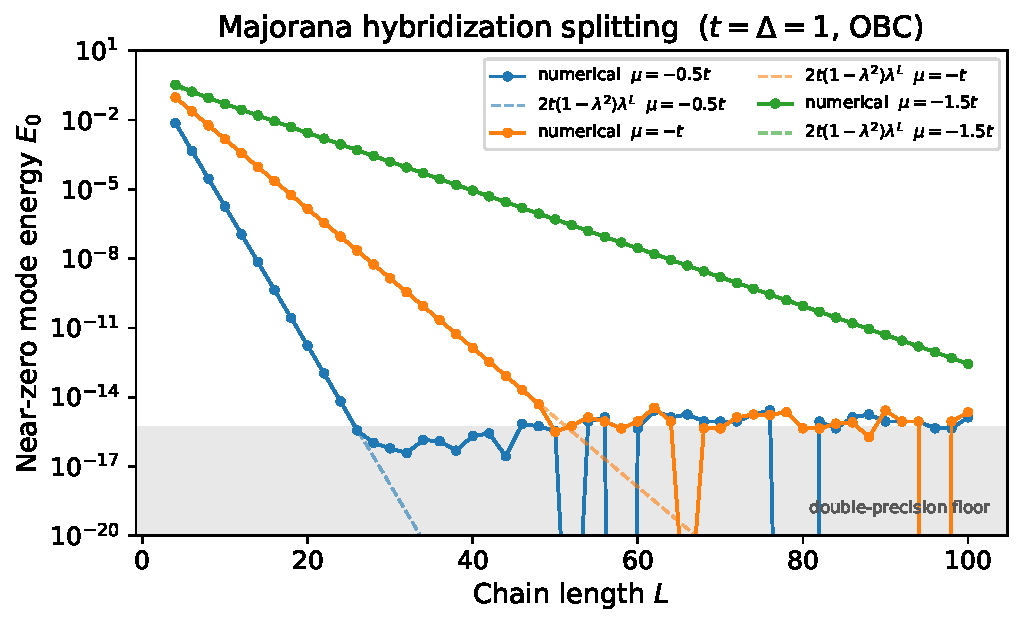
\includegraphics[width=\linewidth]{block1_06_majorana_splitting.pdf}
      \end{center}
    \end{column}
    \begin{column}{0.4\textwidth}
      \textbf{Key result} — at the symmetric point $t=\Delta$:
      \begin{equation}
        E_0(L) \approx 2t\!\left(\frac{|\mu|}{2t}\right)^{\!L} \notag
      \end{equation}
      \begin{itemize}
        \item Straight lines on the semilog scale confirm \textbf{exponential} decay.
        \item Slope $= \ln(|\mu|/2t) = -1/\xi$ measures the \textbf{coherence length} $\xi$.
        \item Smaller $|\mu|$ $\Rightarrow$ faster decay $\Rightarrow$ better protected zero mode.
      \end{itemize}
    \end{column}
  \end{columns}
\end{frame}

% ── Summary ───────────────────────────────────────────────────────────────────
\section{Summary}

\begin{frame}{Block 2 — key takeaways}
  \begin{enumerate}
    \item The BdG matrix is built directly from $\mu$, $t$, $\Delta$ — exact diagonalization gives the full spectrum with no approximations.
    \item OBC spectra show \textbf{near-zero edge modes} in the topological phase — direct numerical confirmation of bulk-boundary correspondence.
    \item Edge modes are \textbf{exponentially localized} with coherence length $\xi = 1/\ln(2t/|\mu|)$.
    \item Majorana splitting decays as $E_0 \sim (|\mu|/2t)^L$ — exponential in $L$, measurable from the semilog slope.
  \end{enumerate}
  \vfill
  \textbf{Next (Block 3):} Jordan–Wigner transform → qubit encoding → quantum circuit for ground-state preparation.
\end{frame}

\end{document}
